% !TEX root = ./Vorlesungsmitschrift AGLA 2.tex  
\lecture{Di 19.05. 10:15}{}
\begin{lemma}
  Sei \( X \) ein euklidischer affiner Raum, \( t\in T(X) \) und \( \tau_t\maps X\to X \) die Translation um \( t \). Seien \( q,q'\in X \) und \( L,L'\subseteq X \) Geraden mit \( L\cap L'\neq \emptyset \). Dann gilt 
  \begin{align*}
    \distance{\tau_t(p)}{\tau_t(q)}&=\distance{p}{q}\text{ und}\\
    \lineangle{\tau_t(L)}{\tau_t(L')}&=\lineangle{L}{L'}.
  \end{align*}
\end{lemma}
\begin{proof}[Beweisidee]
  Verwende
  \begin{equation*}
    \vv{\tau_t(p) \tau_t(q)}\needed{=}\vv{pq},
  \end{equation*}
  \begin{figure}[H]
    \centering
    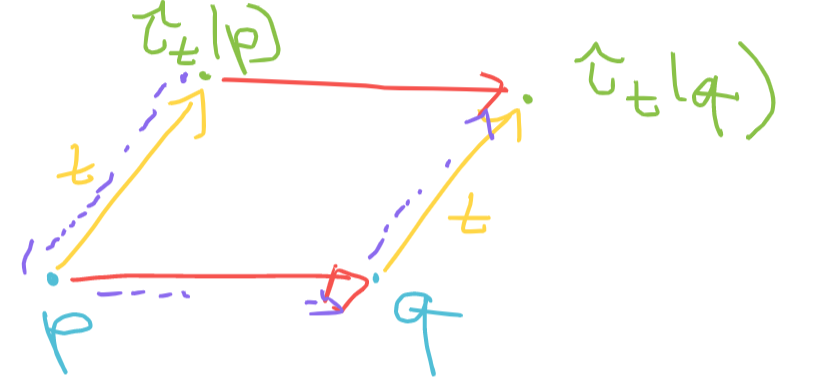
\includegraphics[width=0.5\linewidth]{figures/translation_erhaelt_winkel_beweis_translation_erhaelt_verschiebungen}
    \label{fig:translation_erhaelt_winkel_beweis_translation_erhaelt_verschiebungen}
  \end{figure}
  also
  \begin{equation*}
    \distance{\tau_t(p)}{\tau_t(q)}=\norm*{\vv{\tau_t(p)\tau_t(q)}}=\norm*{\vv{pq}}=\distance{p}{q}
  \end{equation*}
  für beliebige Punkte \( p,q\in X \) und \( t\in T(X) \).
  \begin{figure}[H]
    \centering
    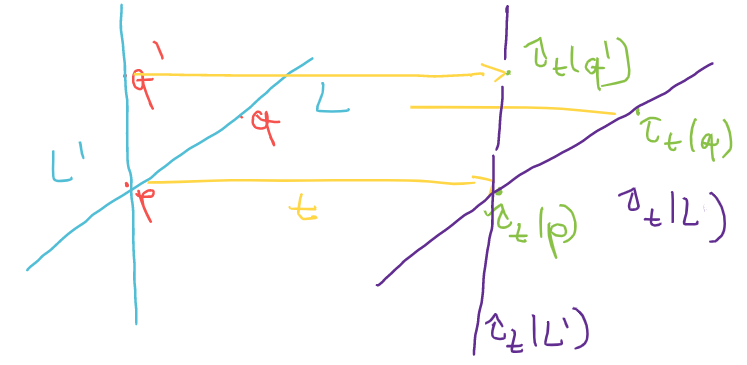
\includegraphics[width=0.5\linewidth]{figures/translation_erhaelt_winkel_beweis_winkel_zwischen_geraden}
    \caption*{Winkel zwischen Geraden \( L,L' \)}
    \label{fig:translation_erhaelt_winkel_beweis_winkel_zwischen_geraden}
  \end{figure}
  \begin{equation*}
    \lineangle{L}{L'}=\arccos \frac{\abs{\scalarproduct{\vv{pq}}{\vv{pq'}}}}{\explain{\norm*{\vv{\tau_t(p)\tau_t(q)}}}{\norm*{\vv{pq}}}\explain[Bigg]{\norm*{\vv{\tau_t(p)\tau_t(q')}}}{\norm*{\vv{pq'}}}}.
  \end{equation*}
\end{proof}
\minisec{also:} Translation um ein Element \( t\in T(X) \) erhält Abstände und Winkel.

Nicht alle affinen Abbildungen haben diese Eigenschaft, \zb \( X=\reals^2 \) mit Standardskalarprodukt.
\begin{figure}[H]
  \centering
  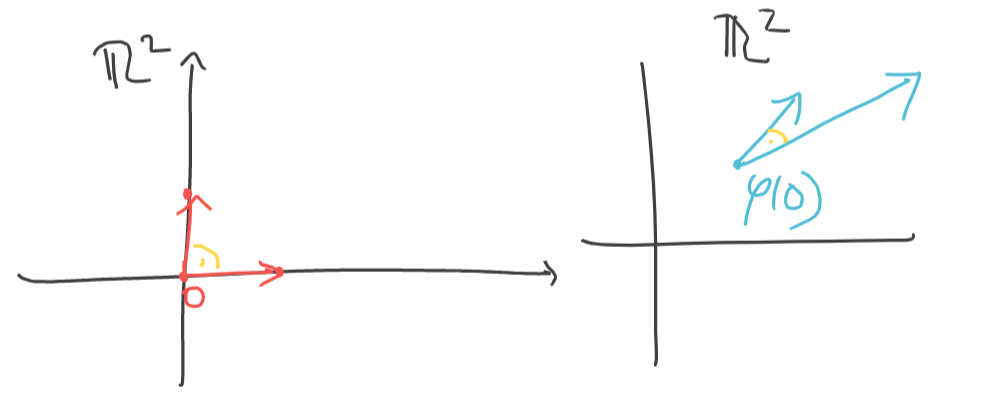
\includegraphics[width=0.5\linewidth]{figures/aehnlichkeiten_gegenbeispiel}
  \caption*{\( \phi\maps X\to X \)}
  \label{fig:aehnlichkeiten_gegenbeispiel}
\end{figure}
\begin{frage*}
  Welche Abbildungen zwischen euklidischen affinen Räumen erhalten Abstände?
\end{frage*}
\begin{definition*}
  Seien \( X,X' \) metrische Räume mit Metriken \( d,d' \) und \( f\maps X\to X' \) eine Abbildung. Wir nennen \( f \) eine \emph{Isometrie}, falls \( \forall p,q\in X \) gilt
  \begin{equation*}
    d'(f(p),f(q))=\distance{p}{q}.
  \end{equation*}
\end{definition*}
\begin{frage*}
  Welche \emph{Abbildungen} zwischen euklidischen affinen Räumen erhalten Abstände?

  \tto Wir können dies Frage auf \emph{affine Abbildungen} reduzieren.
\end{frage*}
\begin{satz}\label{isometrie_affin_und_injektiv}
  Seien \( X,Y \) euklidische affine Räume \( f\maps X\to Y \) eine Isometrie. Dann ist \( f \) \emph{affin} und injektiv.
  \begin{figure}[H]
    \centering
    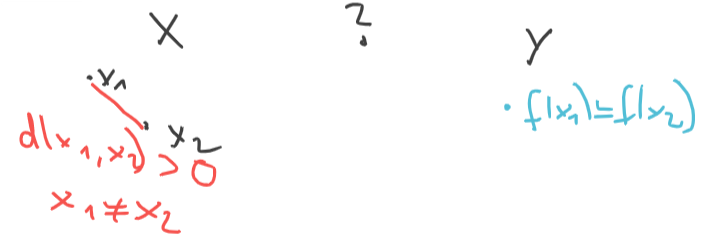
\includegraphics[width=0.5\linewidth]{figures/isometrie_wirklich_injektiv}
    \label{fig:isometrie_wirklich_injektiv}
  \end{figure}
\end{satz}
\begin{proof}
  Sei \( f\maps X\to X \) eine Isometrie und \( p\in X \). Betrachte die Abbildung (mit \( T(X),T(Y) \) Vektorräumen mit Skalarprodukt)
  \begin{equation*}
    F\maps \begin{aligned}[t]
      T(X)&\to T(Y)\\
      \vv{px} &\mapsto \vv{f(p)f(x)}.
    \end{aligned}
  \end{equation*}
  \begin{beweisbehauptung}
    \( F \) ist eine Isometrie.
  \end{beweisbehauptung}
  Seien \( x_1,x_2\in X \).
  \begin{align*}
    \norm*{F(\vv{px_1})-F(\vv{px_2})}_{T(Y)}&=\norm{\vv{f(p)f(x_1)}\underbrace{-\vv{f(p)f(x_2)}}_{=\vv{f(x_2)f(p)}}}_{T(Y)}\\
    &=\norm*{\vv{f(p) f(x_1)}+\vv{f(x_2) f(p)}}_{T(Y)}\\
    &=\norm*{f(x_2)f(x_1)}_{T(Y)}\\
    &=\norm*{\vv{f(x_2) f(x_1)}}_{T(Y)}\\
    &=d_Y(f(x_2), f(x_1))\\
    &\explain{\text{\( f \) ist Isometrie}}{=} d_X(x_2,x_1)=\vv{x_2 x_1}_{T(X)}\\
    &=\norm*{\vv{px_1}-\norm{\vv{px_2}}}_{T(x)}.
  \end{align*}
  \begin{beweisbehauptung}
    Ist \( F \) \emph{linear}, dann ist \( f \) affin. Seien \( x_1,x_2\in X \). Dann gilt 
    \begin{align*}
      F(\vv{x_1 x_2})&=F(\vv{x_1 p}+\vv{p x_2})\\
      &=F(-\vv{px_1}+\vv{px_2})\\
      &\explain{\text{\( F \) ist linear}}{=}-F(\vv{px_1})+F(\vv{px_2})\\
      &=-\vv{f(p)f(x_1)}+\vv{f(p) f(x_2)}\\
      &=\vv{f(x_1)f(x_2)}.
    \end{align*}
    Also ist Abbildung
    \begin{equation*}
      \vv{x_1 x_2}\mapsto \vv{f(x_1) f(x_2)}
    \end{equation*}
    linear!
  \end{beweisbehauptung}
  Es genügt also folgendes Lemma zu beweisen
  \file{Euklidische affine Räume Teil 2}
  \begin{lemma}\label{richtige_isometrie_linear}
    Seien \( V,W \) euklidisch Vektorräume, \( F\maps V\to W \) eine Isometrie mit \( F(0)=0 \). Dann ist \( F \) \emph{linear} und injektiv.
  \end{lemma}
  \begin{proof}[Beweis von Lemma~\ref{richtige_isometrie_linear}]
    \( F \) ist injektiv: Sei \( v',v\in V \) mit \( F(v)=F(v') \). Dann
    \begin{equation*}
      0=d_W(F(v),F(v'))\explain{\text{\( f \) Isometrie}}{=}d_V (v,v'),
    \end{equation*}
    also \( v=v' \).

    Zur Linearität von \( F \): \( F \) ist Isometrie, also gilt \tforall \( v_1,v_2\in V \)
    \begin{equation*}
      \underbrace{\norm*{F(v_1)-F(v_2)}_{d_W(F(v_1),F(v_2))}}=\underbrace{\norm*{v_1-v_2}}_{d_V(v_1,v_2)}.
    \end{equation*}
    Aus \( F(0)=0 \) folgt
    \begin{equation*}
      \norm*{F(v)}=\norm*{v}\quad \forall v\in V
    \end{equation*}
    Berechne für \( v_1,v_2\in V \):
    \begin{equation*}
      \norm*{v_1-v_2}^2=\scalarproduct{v_1-v_2}{v_1-v_2}=\norm*{v_1}^2+\norm*{v_2}^2-2\scalarproduct{v_1}{v_2}.
    \end{equation*}
    Es gilt auch
    \begin{equation*}
      \underbrace{\norm*{F(v_1)-F(v_2)}^2}_{\norm*{v_1-v_2}^2}=\underbrace{\norm*{F(v_1)}^2}_{\norm*{v_1}^2}+\underbrace{\norm*{F(v_2)}^2}_{\norm*{v_2}^2}-2\scalarproduct{F(v_1)}{F(v_2)}.
    \end{equation*}
    Also folgt
    \begin{equation*}
      \scalarproduct{v_1}{v_2}=\scalarproduct{F(v_1)}{F(v_2)}\quad \forall v_1,v_2\in V.
    \end{equation*}
    Seien \( v,v'\in V \).
    \begin{align*}
      \langle \underbrace{F(v+v')-F(v)-F(v')}_{\isittrue{=}0},F(v+v')-F(v)-F(v')\rangle&=\begin{aligned}[t]
        &\scalarproduct{F(v+v')}{F(v+v')}\\
        &-\scalarproduct{F(v+v')}{F(v)}\\
        &-\dotsb\\
        &+\scalarproduct{F(v')}{F(v')}
      \end{aligned}\\
      &=\begin{aligned}[t]
        &\scalarproduct{v+v'}{v+v'}\\
        &-\scalarproduct{v+v'}{v}-\dotsb\\
        &+\scalarproduct{v'}{v'}
      \end{aligned}\\
      &=\scalarproduct{v+v'-v-v'}{v+v'-v-v'} \\
      &=\scalarproduct{0}{0}=0\quad \forall v,v'\in V,
    \end{align*}
    also gilt \( F(v+v')=F(v)+F(v') \). Multiplikation mit Skalaren. Sei \( v\in V \), \( \lambda\in \reals \).
    \begin{align*}
      \scalarproduct{F(\lambda v)-\lambda F(v)}{F(\lambda v)-\lambda F(v)}&=\scalarproduct{F(\lambda v)}{F(\lambda v)}-2\scalarproduct{F(\lambda v)}{\lambda F(v)}\scalarproduct{\lambda F(v)}{\lambda F(V)}\\
      &=\scalarproduct{F(\lambda v)}{F(\lambda v)}-2\lambda \scalarproduct{F(\lambda v)}{F(v)}+\lambda^2\scalarproduct{F(v)}{F(v)}\\
      &=\scalarproduct{\lambda v}{\lambda v}-2\lambda \scalarproduct{\lambda v}{v}+\lambda^2\scalarproduct{v}{v}=(\lambda^2-2\lambda^2+\lambda^2)\scalarproduct{v}{v}\\
      &=0,
    \end{align*}
    also \( F(\lambda v)=\lambda F(v)\quad  \forall \forall \lambda\in\reals\logicspace \forall v\in V \).
  \end{proof}
\end{proof}
\file{Kongruenz}
\begin{definition*}
  Eine Isometrie \( f\maps X\to X \) eines euklidischen affinen Raumes \( X \) nennen wir \emph{Kongruenz} (also nach \thref{isometrie_affin_und_injektiv} immer eine Affinität).
\end{definition*}
\begin{lemma}
  Sei \( f\maps X\to X \) eine Affinität eines euklidischen affinen Raumes \( X \). Dann ist \( f \) eine \emph{Kongruenz} genau dann, wenn die zugehörige lineare Abbildung \( F\maps T(X)\to T(X) \) \emph{orthogonal} ist.
\end{lemma}
\begin{proof}
  \( f  \) ist Isometrie \gdw
  \begin{equation*}
    \distance{f(p)}{f(q)}=\distance{p}{q}\quad \forall p,q\in X,
  \end{equation*}
  \dh \gdw
  \begin{equation*}
    \equalto{\norm*{F(\vv{pq})}}{\norm*{f(p)f(q)}}=\norm{\underbrace{\vv{pq}}_{\in T(X)}} \quad \forall p,q\in X.
  \end{equation*}
  Dies ist äquivalent dazu, dass \( F \) orthogonal ist (also das Skalarprodukt erhält)
\end{proof}
\file{Ähnlichkeiten}
\begin{bemerkung*}
  Im \( \reals^n \) mit Standardskalarprodukt sind Kongruenzen
  \begin{equation*}
    f\maps \reals^n\to \reals^n
  \end{equation*}
  genau durch die Abbildungen der Form
  \begin{equation*}
    f\maps x\mapsto \boxed{f(0)*A\matrixmult x}\quad \forall x\in \reals^n
  \end{equation*}
  gegeben mit \( A\in \orthogonalmatrices{n}{\reals} \) orthogonal, \dh \( \inverse-{A}=\transpose-{A} \). Slogan: \enquote{Kongruenz \( \sim \) orthogonale Abbildung + Translation}.
\end{bemerkung*}
\begin{frage*}
  Kongruenzen erhalten Winkel. Welche \emph{Affinitäten}/ Abbildungen \( f\maps X\to X \) eines euklidischen Raumes \( X \) haben diese Eigenschaft?
\end{frage*}
\begin{beispiel*}
  \( \reals^2 \) mit Standardskalarprodukt.
  \begin{figure}[H]
    \centering
    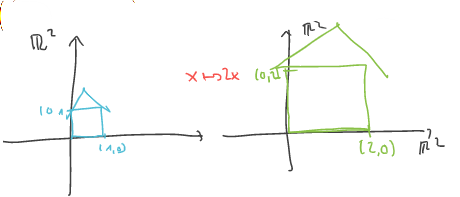
\includegraphics[width=0.5\linewidth]{haus_zu_haus}
    \label{fig:haus_zu_haus}
  \end{figure}
  erhält Winkel, aber nicht Abstände, \dh ist keine Isometrie des \( \reals^2 \).
\end{beispiel*}
\begin{definition*}
  Sei \( X \) ein euklidischer affiner Raum, \( f\maps X\to X \) eine Abbildung. Sei \( \rho\in \reals_{>0} \). Wir nennen \( f  \) eine \emph{Ähnlichkeit} mit (Ähnlichkeits-) Faktor \( \rho \) wenn \tforall  \( p,q\in X \) gilt
  \begin{equation*}
    \distance{f(p)}{f(q)}=\rho\cdot \distance{p}{q}.
  \end{equation*}
\end{definition*}
\begin{korollar*}[aus \thref{isometrie_affin_und_injektiv}]
  Eine Ähnlichkeit \( f\maps X\to X \) eines euklidischen affinen Raumes \( X \) ist eine Affinität.
\end{korollar*}
\begin{proof}
  Sei \( p_0\in X \). Wir definieren eine Affinität
  \begin{equation*}
    \inv{\rho}\maps X\to X
  \end{equation*}
  durch \( \inv{\rho}(p_0)=p_0 \) und
  \begin{equation*}
    \tilde{\rho}\maps \begin{aligned}[t]
      T(X)&\to T(X)\\
      T(X)\ni v&\mapsto \inv{\rho}v.
    \end{aligned}
  \end{equation*}
  \begin{figure}[H]
    \centering
    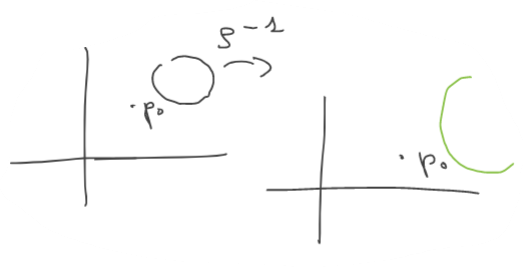
\includegraphics[width=0.5\linewidth]{figures/aehnlichkeiten_sind_affinitaeten_beweis}
    \label{fig:aehnlichkeiten_sind_affinitaeten_beweis}
  \end{figure}
  Wir betrachten die Abbildung
  \begin{equation*}
    \inv{\rho}\circ f\maps X\to X.
  \end{equation*}
  \begin{behauptung*}
    \( \inv{\rho}\circ f \) ist eine Isometrie.
  \end{behauptung*}
  Seien \( p,q\in X \). Dann gilt
  \begin{equation*}
    \distance{\inv{\rho}\circ f(p)}{\inv{\rho}(f(q))}=\norm{\vv{\inv{\rho}\circ f(p) \inv{\rho}\circ f(q)}}
  \end{equation*}
  also
  \begin{align*}
    \distance{\inv{\rho}\circ f(p)}{\inv{\rho}(f(q))}&=\norm*{\inv{\rho}\vv{f(p)f(q)}}\\
    &=\inv{\rho}\norm*{\vv{f(p)f(q)}}\\
    &\explain{\text{\( f \) ist Ähnlichkeit mit Faktor \( \rho \)}}{=}\distance{p}{q},
  \end{align*}
  also ist nach \thref{isometrie_affin_und_injektiv} \( \inv{\rho}\circ f \) injektiv und affin. Damit ist auch \( f \) Affinität.
\end{proof}